\documentclass[10pt]{beamer}
\usetheme[
%%% Modelo modificado para paleta de cores da UNB e apresentação com as logos disponibilizadas pelo próprio site da Universidade.
%%% option passed to the outer theme
%    progressstyle=fixedCircCnt,   % fixedCircCnt, movingCircCnt (moving is deault)
  ]{Feather}
  
% If you want to change the colors of the various elements in the theme, edit and uncomment the following lines

% Change the bar colors:
%\setbeamercolor{Feather}{fg=red!20,bg=red}

% Change the color of the structural elements:
%\setbeamercolor{structure}{fg=red}

% Change the frame title text color:
%\setbeamercolor{frametitle}{fg=blue}

% Change the normal text color background:
%\setbeamercolor{normal text}{fg=black,bg=gray!10}

%-------------------------------------------------------
% INCLUDE PACKAGES
%-------------------------------------------------------

\usepackage[utf8]{inputenc}
\usepackage[english,brazil]{babel}
\usepackage[T1]{fontenc}
\usepackage{helvet}

%-------------------------------------------------------
% DEFFINING AND REDEFINING COMMANDS
%-------------------------------------------------------

% colored hyperlinks
\newcommand{\chref}[2]{
  \href{#1}{{\usebeamercolor[bg]{Feather}#2}}
}

%-------------------------------------------------------
% INFORMATION IN THE TITLE PAGE
%-------------------------------------------------------

\title[] % [] is optional - is placed on the bottom of the sidebar on every slide
{ % is placed on the title page
      \textbf{Estudo segmentação de textos}
}

%\subtitle[Título curto]
%{
%      \textbf{v. 1.0.0}
%}

\author[Matheus Stauffer]
{      Matheus Stauffer Viana de Oliveira \\
      {\ttfamily matheusvostauffer@gmail.com}
}

\institute[]
{
      Departamento de Ciência da Computação\\
      Universidade de Brasília\\
  
  %there must be an empty line above this line - otherwise some unwanted space is added between the university and the country (I do not know why;( )
}

\date{\today}

%-------------------------------------------------------
% THE BODY OF THE PRESENTATION
%-------------------------------------------------------

\begin{document}

%-------------------------------------------------------
% THE TITLEPAGE
%-------------------------------------------------------

{\1% % this is the name of the PDF file for the background
\begin{frame}[plain,noframenumbering] % the plain option removes the header from the title page, noframenumbering removes the numbering of this frame only
  \titlepage % call the title page information from above
\end{frame}}


\begin{frame}{Content}{}
\tableofcontents
\end{frame}


\section{Segmentação de texto}

\begin{frame}[allowframebreaks]{Segmentação de textos}
    \begin{itemize}
        \item Segmentação de textos é a tarefa de extrair segmentos coerentes de texto.
        \item Esses segmentos podem ser categorizados como palavra, sentença, frase ou qualquer unidade de informação dependendo da tarefa de análise envolvida \cite{Irina_text_seg}.
    \end{itemize}
    
    \begin{example}
        Publicações oficiais tais como o Diário Oficial do Distrito Federal (DODF) são fontes de informação sobre todos os atos oficiais do governo. \textcolor{blue}{\textbf{|}} Embora esses documentos sejam ricos em conhecimento, \textcolor{red}{\textbf{||}} analisar esses textos manualmente por especialistas é uma tarefa complexa e inviável considerando o crescente volume de documentos, \textcolor{red}{\textbf{||}} resultado da frequente quantidade de publicações no veículo de comunicação do Governo do Distrito Federal (GDF). \textcolor{blue}{\textbf{|}}
    \end{example}
    
    \begin{figure}
        \centering
        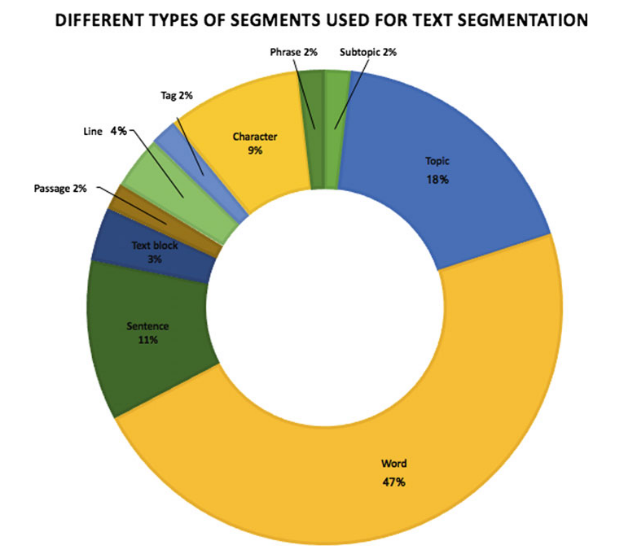
\includegraphics[width=0.65\textwidth]{Feathergraphics/seg_types.png}
        \caption{Tipos de segmentos \cite{Irina_text_seg}}
        \label{fig:seg_types}
    \end{figure}

\end{frame}


\begin{frame}{Segmentação de textos x Modelagem de tópicos}
    \begin{itemize}
        \item Segmentação: determinar as posições onde os (trechos/blocos/segmentos/tópicos/...) mudam em um stream de texto \cite{BarzilayMIT}
    \end{itemize}
    \begin{example}
        Embora esses documentos sejam ricos em conhecimento, [M] \\
        analisar esses textos manualmente ... volume de documentos, [M] \\
        resultado da frequente ... do Distrito Federal (GDF).
    \end{example}
    \flushright \caption{[M] indica mudança de tópico}
\end{frame}

\begin{frame}{Segmentação de textos x Modelagem de tópicos}
    \begin{itemize}
        \item Modelagem de tópicos: objetivo \emph{semântico}. 
    \end{itemize}
    
    \begin{figure}
        \centering
        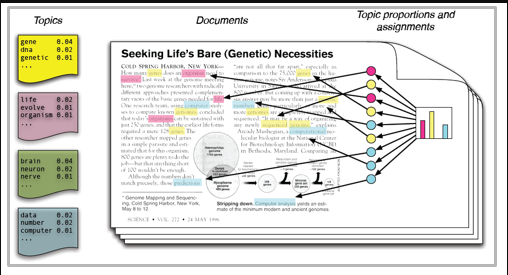
\includegraphics[width=0.7\textwidth]{Feathergraphics/topic_model.png}
        \caption{Exemplo de modelagem de tópicos \footnote{https://www.analyticsvidhya.com/blog/2016/08/beginners-guide-to-topic-modeling-in-python/}}
        \label{fig:my_label}
    \end{figure}
    
\end{frame}

\section{Segmentação de discurso}

\begin{frame}{Segmentação de discurso}

    \begin{itemize}
        \item Uma tarefa relacionada à segmentação de texto que quebra pedações de texto em sub-elementos de uma sentença chamados Unidades Elementares de Discurso (UEDs ou EDUs, em inglês).
        
        \item EDUs são unidades minimais na análise de discurso de acordo com a Teoria da Estrutura Retórica (Mann e Thompson, 1988) \cite{edus_authors}.
        
        \begin{figure}
        \centering
        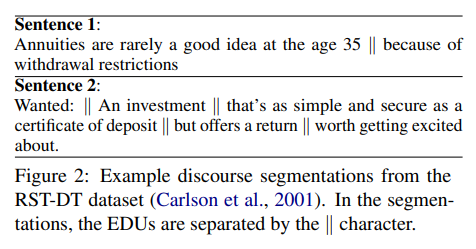
\includegraphics[width=0.5\textwidth]{Feathergraphics/edus_example.png}
        \caption{Exemplo de EDUs \cite{attention_google}}
        \label{fig:edus}
    \end{figure}
    
    \end{itemize}
    
\end{frame}

\section{Abordagens}
\subsection{Segmentação de textos}
\begin{frame}{Abordagens usadas}{Segmentação de textos}
    \begin{itemize}
        \item No alvorecer da pesquisa com segmentação de texto, predominavam abordagens não-supervisionadas, que primavam quantificar coesão léxica em segmentos pequenos de texto \cite{attention_google}.
        
        \item Como é difícil definir e quantificar o que se entende por \emph{coesão léxica}, em geral o termo era designado por/aproximado a `contar repetições de palavras' \cite{attention_google}.
        
        \item No entanto, esse tipo de abordagem sofre com dois principais problemas: é difícil de especializar para um domínio dado e não lida com questões relativas à multi-escala \cite{attention_google}.
        
        \item Nesse sentido, a pesquisa mais recente tem se baseado em propostas supervisionadas, em particular abordagens de redes neurais \cite{attention_google}.
    \end{itemize}
\end{frame}

\subsection{Segmentação de discurso}
\begin{frame}[allowframebreaks]{Abordagens utilizadas}{Segmentação de discurso}
    \begin{itemize}
        \item O problema de segmentação de discurso é, por natureza, mais propenso a encontrar resultados em propostas supervisionadas. Nesse sentido, um desafio é limitação de datasets focados na tarefa; em geral, as abordagens para o problema se pautam em anotadores e recursos externos para ajudar os modelos a generalizarem \cite{attention_google}.
        
        \item Novas propostas recentes se pautam em modelos pré-treinados para obter representações de palavras ou sentenças, como o trabalho de (Li et. al. 2018) \cite{seg_bot}, que propõe dar a um modelo de sequence-to-sequence uma sequência de embeddings GloVe (Pennington et al., 2014) \cite{glove} como entrada para gerar as quebras de EDUs.
        \framebreak
        \item O trabalho de (Lukasik et. al. 2020) \cite{attention_google} introduz novas arquiteturas de modelos baseadas em transformers e embeddings contextuais estilo-BERT para tarefas de segmentação de texto e discurso.
        
        \item Os resultados são promissores: os pesquisadores estabeleceram um novo estado-da-arte.

    \end{itemize}

\end{frame}


\section{References}


\begin{frame}[allowframebreaks]{References}
    \begin{thebibliography}{}

        % Article is the default.
        \setbeamertemplate{bibliography item}[book]
        
        \bibitem{BarzilayMIT}
        Regina Barzilay
        \newblock Text Segmentation (2005)
        \newblock \url{https://ocw.mit.edu/courses/electrical-engineering-and-computer-science/6-864-advanced-natural-language-processing-fall-2005/lecture-notes/lec13.pdf}
        
        \bibitem{Irina_text_seg}
        Irina Pak e Phoey Lee Teh
        \newblock Text Segmentation Techniques - a critical review (2018)
        \newblock \url{https://www.researchgate.net/publication/321227216_Text_Segmentation_Techniques_A_Critical_Review}
        
        \bibitem{Mizra_topic_modeling}
        Hemant Misra, François Yvon, Olivier Cappé e Joemon Jose
        \newblock Text segmentation: A topic modeling perspective (2019)
        \newblock \url{https://hal.archives-ouvertes.fr/hal-01960703/document}
        
        \bibitem{Riedl_topic_modeling}
        Martin Riedl e Chris Biemann
        \newblock How Text Segmentation Algorithms Gain from Topic Models (2012)
        \newblock \url{https://www.aclweb.org/anthology/N12-1064.pdf}
        
        \bibitem{wallach_topic_modeling}
        Hanna M. Wallach
        \newblock Topic Modeling: Beyond Bag-of-Words (2006)
        \newblock \url{https://people.cs.umass.edu/~wallach/talks/beyond_bag-of-words.pdf}
        
        \bibitem{attention_google}
        Michal Lukasik, Boris Dadachev, Gonçalo Simões, Kishore Papineni\newblock Text Segmentation by Cross Segment Attention
        \newblock \url{https://arxiv.org/pdf/2004.14535.pdf}
        
        \bibitem{edus_authors}
        William C Mann e Sandra A Thompson
        \newblock Rhetorical structure theory: Toward a functional theory of text organization (1988)
        \newblock Journal for the Study of Discourse, 8(3):243–281.
        
        \bibitem{seg_bot}
        Jing Li, Aixin Sun, and Shafiq Joty. 
        \newblock Segbot: A generic neural text segmentation model with pointer network (2018). 
        \newblock In Proceedings of the Twenty-Seventh International Joint Conference on Artificial Intelligence, IJCAI-18, pages 4166–4172. International Joint Conferences on Artificial Intelligence Organization.
        
        \bibitem{glove}
        Jeffrey Pennington, Richard Socher, and Christopher Manning. \newblock Glove: Global vectors for word representation (2014)
        \newblock In Proceedings of the 2014 Conference on Empirical Methods in Natural Language Processing (EMNLP), pages 1532–1543, Doha, Qatar. Association for Computational Linguistics.
        
    

    \end{thebibliography}
\end{frame}




\end{document}